\documentclass[11pt]{article}
\usepackage[a4paper,margin=19mm]{geometry}
\usepackage{fontspec}
\setmainfont{lmroman10-regular.otf}
\usepackage{amsmath,amssymb,amsthm,mathtools,xcolor,graphicx,hyperref}
\hypersetup{hidelinks}
\numberwithin{equation}{section}
\newtheorem{theorem}{Theorem}[section]
\newtheorem{lemma}[theorem]{Lemma}
\newtheorem{proposition}[theorem]{Proposition}
\newtheorem{corollary}[theorem]{Corollary}
\newtheorem{claim}[theorem]{Claim}
\newtheorem{fact}[theorem]{Fact}
\newtheorem{conjecture}[theorem]{Conjecture}
\theoremstyle{definition}
\newtheorem{definition}[theorem]{Definition}
\newtheorem{example}[theorem]{Example}
\newtheorem{remark}[theorem]{Remark}
\newtheorem{question}[theorem]{Question}
\theoremstyle{plain}
\newcommand{\C}{\mathbb C}
\newcommand{\R}{\mathbb R}
\newcommand{\Q}{\mathbb Q}
\newcommand{\Z}{\mathbb Z}
\newcommand{\N}{\mathbb N}
\newcommand{\eee}{\mathrm e}
\newcommand{\cclass}[1]{\textsf{#1}}
\newcommand{\cproblem}[1]{\textsc{#1}}
\newcommand{\ie}{i.\,e.}
\newcommand{\Ie}{I.\,e.}
\newcommand{\eg}{e.\,g.}
\newcommand{\Eg}{E.\,g.}
\newcommand{\phd}{Ph.\,D.}
\newcommand{\msc}{M.\,S.}
\newcommand{\bsc}{B.\,S.}
\newcommand{\expref}[2]{\hyperref[#2]{#1~\ref{#2}}}
\newcommand{\expeqref}[2]{\hyperref[#2]{#1~\eqref{#2}}}
\newcommand{\exprefsilent}[2]{\hyperref[#2]{#1}}
\providecommand{\etal}{et~al.}
\usepackage{eprint}
\usepackage{xspace}
\usepackage{tikz}
\usepackage{braket}
\usetikzlibrary{calc}

%
\newcommand{\pav}{\ensuremath{\mathcal{A}_v}}
\newcommand{\column}{\ensuremath{\textup{column}}}
\newcommand{\row}{\ensuremath{\textup{row}}}
\newcommand{\toprow}{\ensuremath{\textup{toprow}}}
\newcommand{\bottomrow}{\ensuremath{\textup{bottomrow}}}
\newcommand{\dist}{\ensuremath{\textup{columndist}}}
\newcommand{\cost}{\ensuremath{\textup{cost}}}

%
%
%
\newcommand{\Nat}{\ensuremath{\mathbb{N}}}

\newcommand{\calA}{\ensuremath{\mathcal{A}}}
\newcommand{\calI}{\ensuremath{\mathcal{I}}}
\newcommand{\calT}{\ensuremath{\mathcal{T}}}
\newcommand{\calU}{\ensuremath{{\mathcal{U}}}}
\newcommand{\Hamarray}{\ensuremath{\textup{HamArray}}}
\newcommand{\Prob}{\ensuremath{\textup{Pr}}}
\newcommand{\expected}[1]{\ensuremath{\mathbb{E}[#1]}}
\newcommand{\expecteddisplay}[1]{\ensuremath{\mathbb{E}\left[#1\right]}}
\newcommand{\Ham}[1]{\ensuremath{\textup{Ham}(#1)}}
\newcommand{\ED}[1]{\ensuremath{\textup{Edit}(#1)}}
\newcommand{\ball}[1]{\ensuremath{\textup{Ball}(#1)}}
%
\newcommand{\Vsum}{\ensuremath{\textup{Sum}}}
\newcommand{\vsum}{\ensuremath{\textup{sum}}}
\newcommand{\LCSt}{\ensuremath{\textup{LCS}(F,S_t)}}
\newcommand{\HAMt}{\ensuremath{\textup{Ham}(F,S_t)}}

\newcommand{\lit}{large information transfer\xspace}
\newcommand{\MFL}{\ensuremath{M_{F,\ell}}}

\newcommand{\HamInt}[1]{\ensuremath{D{[#1]}}}
\newcommand{\T}{\ensuremath{T}}
\newcommand{\UInt}[1]{\ensuremath{U{[#1]}}}
\newcommand{\UcompInt}[1]{\ensuremath{U{[#1]^\textup{c}}}}
\newcommand{\Ufix}{\ensuremath{U_{\textup{fix}}{[t_0,t_1]^\textup{c}}}}

%
\newcommand{\Xv}{\ensuremath{U_v}}
\newcommand{\Xvknown}{\ensuremath{\widetilde{U}_v}}
%
\newcommand{\Xvfix}{\ensuremath{\widetilde{u}_v}}
\newcommand{\Yv}{\ensuremath{A_v}}
%
\newcommand{\IT}{\ensuremath{IT}}
\newcommand{\vitset}{\ensuremath{\mathcal{I}_v}}
\newcommand{\vit}{\ensuremath{I_v}}
\newcommand{\vtime}{\ensuremath{R_v}}
\newcommand{\vcap}{\ensuremath{r_v}}
\newcommand{\venc}{\ensuremath{Z_v}}
\newcommand{\entfac}{\ensuremath{f}}

%

\renewcommand{\S}{{\ensuremath{S}}} %
\newcommand{\U}{{\ensuremath{U}}} %
\newcommand{\n}{{\ensuremath{n}}} %

\newcommand{\arrive}{\ensuremath{\textsc{update}}}

\newcommand{\Cbig}{\ensuremath{\widetilde{C}}}
\newcommand{\Cbigprime}{\ensuremath{\widetilde{C}'}}
\newcommand{\cbig}{\ensuremath{\widetilde{c}}}
\newcommand{\cbigI}{\ensuremath{\widetilde{c_1}}}
\newcommand{\cbigII}{\ensuremath{\widetilde{c_2}}}
\newcommand{\cbigprime}{\ensuremath{\widetilde{c}\,'}}

\newcommand{\ELL}{\ensuremath{\mu}}
\newcommand{\ps}{\ensuremath{\rho}}
\newcommand{\psymb}{\ensuremath{\star}}
\newcommand{\psymbb}{\ensuremath{\star}}

\newcommand{\tsymb}{\ensuremath{\diamond}}

\newcommand{\wildcard}{\ensuremath{\star}}

\newcommand{\alignment}[1]{{\small{\textcircled{\scriptsize #1}}}}


%
%
%
\newcommand{\expect}[1]{\mathbb{E}\left[{#1}\right]}
\newcommand{\expectinline}[1]{\mathbb{E}[{#1}]}
\newcommand{\twodots}{\ensuremath{\,.\,.\,}}

%
%
%
\newcommand{\insertdiagram}[1]{\includegraphics[scale=0.82]{#1}}
\newcommand{\Patrascu}{P{\v a}tra{\c s}cu\xspace}

%
%

\newcommand{\inserttreefigure}{
\newcommand{\nodefont}{\scriptsize}
\begin{figure}[t]
\centering
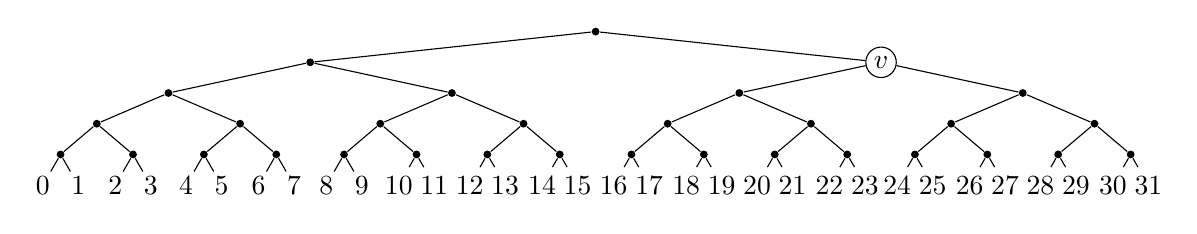
\begin{tikzpicture}[level distance=3.9mm]
\tikzstyle{every node}=[fill=black!100,circle,inner sep=1pt]
\tikzstyle{level 1}=[sibling distance=72.5mm]
\tikzstyle{level 2}=[sibling distance=36mm]
\tikzstyle{level 3}=[sibling distance=18.2mm]
\tikzstyle{level 4}=[sibling distance=9.2mm]
\tikzstyle{level 5}=[sibling distance=4.5mm,set style={{every node}+=[fill=white!15]}]
\node {}
    child {node {}
        child {node {}
            child {node {}
                child {node {}
                    child {node {\nodefont 0}}
                    child {node {\nodefont 1}}
                }
                child {node {}
                    child {node {\nodefont 2}
                    }
                    child {node {\nodefont 3}
                    }
                }
            }
            child {node {}
                child {node {}
                    child {node {\nodefont 4}}
                    child {node {\nodefont 5}}
                }
                child {node {}
                    child {node {\nodefont 6}
                    }
                    child {node {\nodefont 7}
                    }
                }
            }
        }
        child {node {}
            child {node {}
                child {node {}
                    child {node {\nodefont 8}}
                    child {node {\nodefont 9}}
                }
                child {node {}
                    child {node {\nodefont 10}
                    }
                    child {node {\nodefont 11}
                    }
                }
            }
            child {node {}
                child {node {}
                    child {node {\nodefont 12}}
                    child {node {\nodefont 13}}
                }
                child {node {}
                    child {node {\nodefont 14}
                    }
                    child {node {\nodefont 15}
                    }
                }
            }
        }
    }
    child {node[fill=black!00,circle,draw,inner sep=1.5pt] {$v$}
        child {node {}
            child {node {}
                child {node {}
                    child {node {\nodefont 16}}
                    child {node {\nodefont 17}}
                }
                child {node {}
                    child {node {\nodefont 18}
                    }
                    child {node {\nodefont 19}
                    }
                }
            }
            child {node {}
                child {node {}
                    child {node {\nodefont 20}}
                    child {node {\nodefont 21}}
                }
                child {node {}
                    child {node {\nodefont 22}
                    }
                    child {node {\nodefont 23}
                    }
                }
            }
        }
        child {node {}
            child {node {}
                child {node {}
                    child {node {\nodefont 24}}
                    child {node {\nodefont 25}}
                }
                child {node {}
                    child {node {\nodefont 26}
                    }
                    child {node {\nodefont 27}
                    }
                }
            }
            child {node {}
                child {node {}
                    child {node {\nodefont 28}}
                    child {node {\nodefont 29}}
                }
                child {node {}
                    child {node {\nodefont 30}
                    }
                    child {node {\nodefont 31}
                    }
                }
            }
        }
    };
\end{tikzpicture}

%\insertdiagram{tree}
\caption{\label{fig:tree}An information transfer tree $\calT$ with $n=32$ leaves. For the node labelled $v$, the arrival times $t_0=16$, $t_1=23$ and $t_2=31$.}
\end{figure}
}




\makeatother
\providecommand{\definitionname}{Definition}
\providecommand{\lemmaname}{Lemma}
\providecommand{\problemname}{Problem}
\providecommand{\theoremname}{Theorem}


%
\newcommand{\Xc}{\ensuremath{X[t_0,t_1]^\textup{c}}}
\newcommand{\Xfix}{\ensuremath{X^{\textup{fix}}{[t_0,t_1]^\textup{c}}}}
\newcommand{\VB}{\ensuremath{V}}      %


%
%
%

\newtheorem{problem}[theorem]{Problem}
